\documentclass[journal=esthag,manuscript=article]{achemso}
%%%%%%%%%%%%%%%%%%%%%%%%%%%%%%%%%%%%%%%%%%%%%%%%%%%%%%%%%%%%%%%%%%%%%
%% Place any additional packages needed here.  Only include packages
%% which are essential, to avoid problems later. Do NOT use any
%% packages which require e-TeX (for example etoolbox): the e-TeX
%% extensions are not currently available on the ACS conversion
%% servers.
%%%%%%%%%%%%%%%%%%%%%%%%%%%%%%%%%%%%%%%%%%%%%%%%%%%%%%%%%%%%%%%%%%%%%
\usepackage[T1]{fontenc}       % Use modern font encodings
\usepackage[utf8]{inputenc}
\usepackage{amsmath}
\usepackage{enumerate}

\usepackage{todonotes}

%%%%%%%%%%%%%%%%%%%%%%%%%%%%%%%%%%%%%%%%%%%%%%%%%%%%%%%%%%%%%%%%%%%%%
%% If issues arise when submitting your manuscript, you may want to
%% un-comment the next line.  This provides information on the
%% version of every file you have used.
%%%%%%%%%%%%%%%%%%%%%%%%%%%%%%%%%%%%%%%%%%%%%%%%%%%%%%%%%%%%%%%%%%%%%
%%\listfiles

%%%%%%%%%%%%%%%%%%%%%%%%%%%%%%%%%%%%%%%%%%%%%%%%%%%%%%%%%%%%%%%%%%%%%
%% Place any additional macros here.  Please use \newcommand* where
%% possible, and avoid layout-changing macros (which are not used
%% when typesetting).
%%%%%%%%%%%%%%%%%%%%%%%%%%%%%%%%%%%%%%%%%%%%%%%%%%%%%%%%%%%%%%%%%%%%%
%% \newcommand*\mycommand[1]{\texttt{\emph{#1}}}


%%%%%%%%%%%%%%%%%%%%%%%%%%%%%%%%%%%%%%%%%%%%%%%%%%%%%%%%%%%%%%%%%%%%%
\author{Eduard Szöcs}
\affiliation[Institute for Environmental Sciences]{Institute for Environmental Sciences, University of Koblenz-Landau, Germany}
\email{szoecs@uni-landau.de}
\phone{+49 (0)6341 280 31552}

\author{Marvin Brinke}
\affiliation[German Federal Institute of Hydrology]{German Federal Institute of Hydrology (BfG), Koblenz, Germany}

\author{Bilgin Karaoglan}
\affiliation[German Federal Environmental Agency]{Federal Environmental Agency (UBA), Dessau-Roßlau, Germany}

\author{Ralf B. Schäfer}
\affiliation[University Koblenz-Landau]{Institute for Environmental Sciences, University of Koblenz-Landau, Germany}


%%%%%%%%%%%%%%%%%%%%%%%%%%%%%%%%%%%%%%%%%%%%%%%%%%%%%%%%%%%%%%%%%%%%%
\title[Pesticides small streams]{Pesticides in small agricultural streams in Germany}
% \abbreviations{mo, neon, ra, tu, fw}
\keywords{Monitoring, Neonicotinoid, Risk Assessment Toxic Units, Freshwater}
% RAC, 

%%%%%%%%%%%%%%%%%%%%%%%%%%%%%%%%%%%%%%%%%%%%%%%%%%%%%%%%%%%%%%%%%%%%%
\begin{document}
%%%%%%%%%%%%%%%%%%%%%%%%%%%%%%%%%%%%%%%%%%%%%%%%%%%%%%%%%%%%%%%%%%%%%
%% The "tocentry" environment can be used to create an entry for the
%% graphical table of contents. It is given here as some journals
%% require that it is printed as part of the abstract page. It will
%% be automatically moved as appropriate.
%%%%%%%%%%%%%%%%%%%%%%%%%%%%%%%%%%%%%%%%%%%%%%%%%%%%%%%%%%%%%%%%%%%%%
\begin{tocentry}

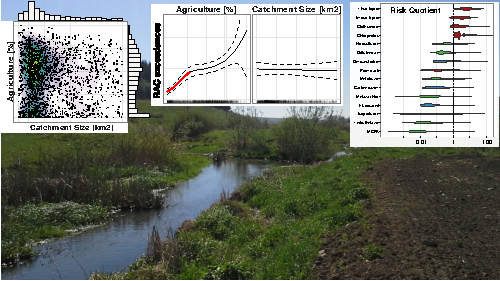
\includegraphics[width=0.7\textwidth]{abstract.pdf}

\end{tocentry}


%%%%%%%%%%%%%%%%%%%%%%%%%%%%%%%%%%%%%%%%%%%%%%%%%%%%%%%%%%%%%%%%%%%%%
\begin{abstract}
% 150-200 words
Small streams are important refugia for biodiversity.
In agricultural areas, they may be at high risk of pesticide pollution. However, most related studies have been limited to a few streams on the regional level, hampering extrapolation to larger scales.
In Germany, pesticide monitoring is performed by the federal states as part of water quality surveillance. 
\end{abstract}


%% -------------------------------------------------------------------------
\section{Introduction}
More than 50\% of the total land area in Germany are used by agriculture \citep{statistisches_bundesamt_bodenflache_2014}.
In the year 2014 more than 45,000 tonnes of 766 authorized pesticides were sold for application on this area \citep{bundesamt_fur_verbraucherschutz_und_lebensmittelsicherheit_absatz_2015}.
The applied pesticides may enter surface waters via spray-drift, edge-off-field run-off or drainage \citep{stehle_probabilistic_2013,schulz_comparison_2001,liess_determination_1999}.
Especially run-off after heavy precipitation events has been shown to be one of the major input routes \citep{schulz_field_2004}.
Once entered the surface waters they may have adverse effects on biota and ecosystem functioning \citep{schafer_thresholds_2012}.

\citet{malaj_organic_2014} analyzed data supplied to the European Union (EU) in the context of the Water Framework Directive (WFD) and showed that most European water bodies are at risk from pesticides.
\citet{stehle_pesticide_2015} compiled 1566 measured concentrations of 23 insecticides in the EU from scientific publications. 
They found that many of these measurements exceed regulatory acceptable concentrations (RAC).
Both studies indicate that pesticides might be a threat to biodiversity in the European union. 
However, theses studies reflect only a small part of available data and it is unclear how representative they are:
For Germany the study of \citet{malaj_organic_2014} lists only 175 sites and \citet{stehle_pesticide_2015} only 138 measurements, although there might my much more data available from national monitoring programs. %175 estimated from digitized figure C.3 in Malaj 2014, Stehle: Table 2.

Small water bodies (SWB) comprise a major fraction of streams \citep{nadeau_hydrological_2007}, accommodate a higher proportion of biodiversity compared to larger freshwater systems \citep{davies_comparison_2008, biggs_report_2014} and play an important role in recolonization of disturbed downstream reaches \citep{liess_analyzing_2005, orlinskiy_forested_2015}.
However, SWB might be also at high risk of pesticide contamination from adjacent agricultural areas and lower dilution potential \citep{schulz_field_2004}.
It has been show that SWB are more polluted than bigger streams \citep{stehle_pesticide_2015,schulz_field_2004}.
Despite their relevance only a small fraction of studies were conducted on pesticide pollution of SWB \todo{citation Lorenz et al.}, with only few large scale studies.

We compiled a large data set with chemical monitoring data for Germany and aimed to answer the following research questions: 

\begin{enumerate}[(i)]
	\item Can the currently available monitoring data be used for a representative description of the pollution situation?
	\item Are there thresholds for agricultural land use above pesticide pollution becomes apparent?
	\item Are there thresholds of stream size below pesticide pollution becomes apparent
	\item  How polluted are small agricultural streams in Germany and which pesticides are most important? 
\end{enumerate}




%% -------------------------------------------------------------------------
\section{Methods}
\subsection{Data compilation}
We compiled pesticide monitoring data from sampling sites with catchment sizes $\mathrm{< 100km^2}$ for the years 2005 to 2015 from all 13 non-city federal states of Germany (see supplemental table S1 for the abbreviations of federal state names). 
We homogenized and unified all data from the states into a common database.
We implemented a robust and reproducible data cleaning workflow (see supplement for details on the data processing workflow) \citep{poisot_best_2015}.
Nevertheless, parts of the dataset are proprietary and cannot be shared here.

Given the relevance of precipitation in causing runoff events, we identified chemical samples taken during heavy rainfall events.
We performed a spatio-temporal intersection of sampling events with gridded daily precipitation data available the German Weather service \citep{rauthe_central_2013}. 
We performed the intersection for the actual sampling date and the day before.


\subsection{Characterization of chemical pollution}
We characterized pesticide pollution using regulatory acceptable concentrations (RAC) \citep{brock_linking_2010}.
RACs are derived during pesticide authorization and no unacceptable ecological effect are expected if the environmental concentration remains below this concentration.
The German Federal Environmental Agency provided RACs for the 105 compounds with highest detection rates (Supplement, Table S2). 
We expressed RACs as Risk Quotient (RQ):

\begin{equation}
RQ_i = \frac{C_i}{RAC_i}
\end{equation}

Where $C_i$ is the concentration of a compound $i$ in a sample.


\subsection{Characterization of catchments}
We compiled a total of 3,049 sampling sites with pesticide measurements.
We delineated catchments upstream for each of the sampling sites using a digital elevation model (DEM) \citep{eea_digital_2013} and the multiple flow direction algorithm \citep{holmgren_multiple_1994} as implemented in GRASS GIS 7 \citep{neteler_grass_2012}.
Catchment delineation was manually checked for accuracy by comparison with a stream network provided by the government.
The delineation algorithm produced only for 30\% of the sites accurate results.
For the rest we were able to compile catchment size data from authorities (47\% of sites) or drainage basins per stream segment provided by authorities (13\% of sites).
For 10\% of the sites we were not able to compile catchment size data.
For each derived catchment (either from DEM or drainage basins) we calculated the relative cover (in \%) with agricultural areas based on Official Topographical Cartographic Information System (ATKIS) of the land survey authorities \citep{adv_atkis_2016}.
We additionally used agricultural cover data provided by authorities (18\% of sites), which resulted to 21\% of sites with missing agricultural cover data. 
For 78\% of the sites both, the proportion of agricultural landuse and catchment size were available.
% see do_overview.R for numbers


\subsection{Statistical analyses}
All data-processing and analyses were performed using R \citep{r_core_team_r:_2016}.
To display differences in the spectra of analyzed compounds between federal states we used Multidimensional Scaling (MDS) based on Jaccard dissimilarity in conjunction with complete linkage hierarchical clustering using the vegan package \citep{oksanen_vegan:_2016}.
We expected non-linear responses to agriculture and catchment size and therefore, used generalized additive models (GAM) to identify relationships \citep{fewster_analysis_2000}.
We modeled the number of RAC exceedances as:

\begin{align}
\begin{split}
  No_i \sim NB(\mu_i, k) \\
  E(No_i) = \mu_i~and~Var(No_i) = \mu_i + \frac{\mu_i^2}{k} \\
  log(\mu_i)= \beta_0 + f_1(Agri_i) + f_2(Size_i) + log(n_i) \\
\end{split}
\end{align}

where $No_i$ is the observed number of exceedances at site $i$. 
The proportion of agriculture within the catchment ($Agri_i$) and the catchment size of the site ($Size_i$) were used as predictors. 
We modeled $No_i$ as resulting from a negative binomial distribution ($NB$).
The number of sampling events per site ($n_i$) was as an offset to account different sampling efforts at a site and is equivalent to modeling the rate of exceedances. 
$f_1$ and $f_2$ are smoothing functions using thin plate regression splines \citep{wood_thin_2003}.
The degree of smoothness was estimated using restricted maximum likelihood (REML) during model fitting process \citep{wood_fast_2011}.
We used point-wise 95\% Confidence Intervals of the first derivative of the fitted smooth to check if there are regions of statistically significant changes.
GAMs were fitted using the mgcv package \citep{wood_fast_2011}.
\todo{precipitation stats?}



%% -------------------------------------------------------------------------
\section{Results}
\subsection{Overview of the compiled data}

The compiled dataset comprised only few standing waters (58 sites) and the majority of samples (91\%) where taken via grab sampling.  % see clean.R for numbers
9\% of samples from 33 sites were taken as composite samples of different durations.
Therefore, we report only results of grab samples from streams. 
The analyzed dataset comprised 2,918,604 pesticide measurements of 42,236 samples in 3,049 sampling sites.  %see do_overview.R for numbers.
We found large differences in the number of sampling sites between federal states (Figure \ref{fig:fig1} and Supplement, Table S1).

\begin{figure}[ht]
  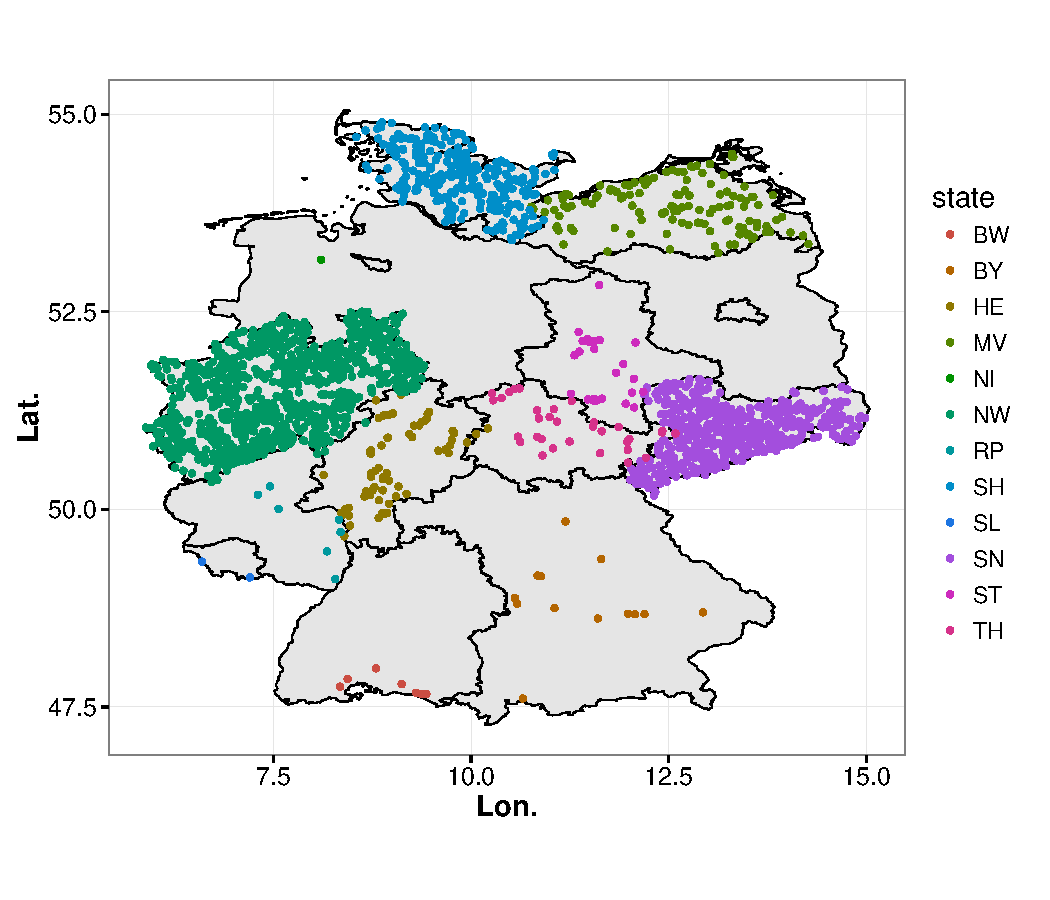
\includegraphics[width=0.6\textwidth]{figure1.pdf}
  \caption{Spatial distribution of the 3109 sampling sites. Colour codes different federal states, see supplemental table S1 for abbreviations.}
  \label{fig:fig1}
\end{figure}

In total 484 different compounds used as pesticides and their metabolites were measured at least once (Supplement, Table S2 \todo{remove LC50 and MAC-EQS from table!}). 
Most of the compounds were herbicides (179), followed by insecticides (117) and fungicides (109).
Only 5.5\% (160,800) of all measurements were detects above the limit of quantification (LOQ).
We found substantial differences in the spectra of analyzed compounds between federal states (Figure \ref{fig:fig2} and Supplement Figure S2).
Hierarchical clustering revealed three groups:

\begin{enumerate}[i)]
	\item with less then 100 compounds (SL, ST and TH)
	\item with medium sized spectra
	\item with a big and distinct spectrum (RP and NI)
\end{enumerate}


\begin{figure}[ht]
  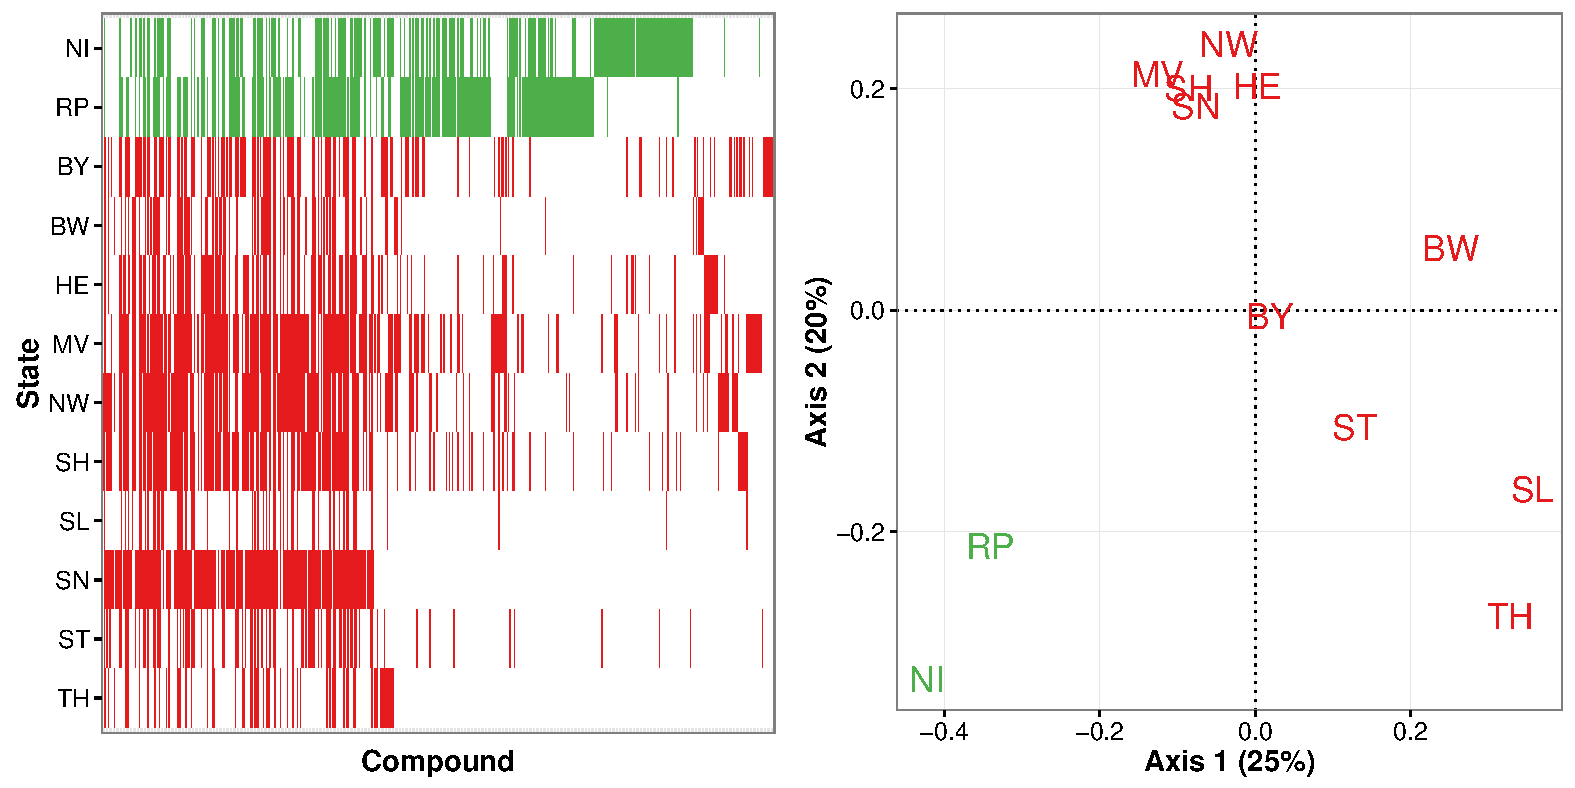
\includegraphics[width=\textwidth]{figure2.pdf}
  \caption{Compound spectra of the different federal states. Left: Barcode plot - Each vertical line is an analysed compound. Right: MDS ordination. 
  Colors according to three groups determined by hierarchical clustering (see Supplement Figure S2).}
  \label{fig:fig2}
\end{figure}


\todo{precipitation section should be moved / more}
The spatio-temporal intersection revealed that 5\% of the samples were taken at or after days with rainfall events greater than 10mm / day (Supplement, Figure S3).




%%%%%%%%%%%%%%%%%%%%%%%%%%%%%%%%%%%%%%%%%%%%%%%%%%%%%%%%%%%%%%%%%%%%%
\begin{acknowledgement}
The authors thank the federal state authorities for providing chemical monitoring data and the German Federal Environmental Protection Agency (UBA) for funding a related project (FKZ 3714 67 4040 / 1). 
\end{acknowledgement}


%%% Word count
% abstract    :
% 3 big(600)  : 1800
% 2 small(300): 600
% text body   : 3000 
% ackno       : 24
% ======================================
% total       : 

%%%%%%%%%%%%%%%%%%%%%%%%%%%%%%%%%%%%%%%%%%%%%%%%%%%%%%%%%%%%%%%%%%%%%
\begin{suppinfo}
The following files are available free of charge.
\begin{itemize}
  \item Supplemental\_Materials.pdf : Supplemental Materials (Figures, Tables, Models).
\end{itemize}
\end{suppinfo}


%%%%%%%%%%%%%%%%%%%%%%%%%%%%%%%%%%%%%%%%%%%%%%%%%%%%%%%%%%%%%%%%%%%%%
\bibliography{references}

\end{document}
